\section{Estimating Mixture-of-Expert (\moe) \flops}
\label{app:train_inference_cost}

Similar to prior work on scaling laws (e.g., ~\citet{kaplan_scale,hoffmann2022training,ludziejewski2024scaling}), we use theoretical FLOP estimates as proxies for training and inference costs of language models. 
In this section, we (a) outline our methodology for estimating FLOPs for \moes and (b) show that the proposed estimator closely approximates empirical FLOPs of large-scale \moes.

\paragraph{Setup and notation.} 
Consider an \moe model with $n_{\text{layers}}$ \moe layers, each with an embedding dimension of $d_{\text{model}}$. 
We denote the number of total experts and active experts in each \moe layer by $E_{\text{total}}$ and $E_{\text{active}}$ respectively. Following~\citet{ludziejewski2024scaling}, we let $G$ denote the \moe granularity, which defaults to $1$ and controls the size of each expert relative to the size of a feed-forward layer in an equivalent dense transformer. 
In order to change sparsity in a more granular manner, we treat the number of active experts as an independent variable that does not scale with granularity $G$.
In our experiments, we use a vocabulary size $n_{\text{vocab}} = 50,432$, a context length $n_{\text{ctx}}$ of $2048$, and GLU modules (Gated Linear Units)~\citep{shazeer2017} over feed-forward modules as the architecture of choice for \moe experts. 
We also set the (a) hidden dimension of each GLU expert $d_{\text{ffn}}$ to $4 \cdot d_{\text{model}}$ and (b) instantiate \moes where the number of attention heads $n_{\text{heads}}$ times the dimensionality for each head $d_{\text{head}}$ equals $d_{\text{model}}$, i.e., $n_{\text{heads}} d_{\text{head}} = d_{\text{model}}$.

\paragraph{Estimating module-specific FLOPs.} To estimate the FLOPs of a given \moe model, we first individually estimate the FLOPs per token incurred by a forward \emph{and} backward pass through every module in \moes. 
Then, we  aggregate these estimates to obtain the final estimator for the FLOPs per token incurred by a forward \emph{and} backward pass through the model.

Like in prior work on scaling laws~\citep{kaplan_scale,hoffmann2022training}, we take a two-step approach to estimate module-specific FLOPs. 
Given a module, we first estimate the number of parameters in the module and then scale this with an appropriate constant corresponding to the number of add-multiply operations per parameter through a forward and backward pass of the given module.  
We also omit non-leading terms such as non-linearities, biases, and layer normalization in our estimation. We estimate the FLOPs per token for attention modules, \moe routers, \moe experts, and the final un-embedding layer as follows:
\begin{enumerate}[left=10pt,itemsep=2pt]
    \item \textbf{Attention module.} We estimate the FLOPs incurred via the QKV (and final) projections, attention logits, and attention values of all heads in a multi-head attention module as follows.
    \begin{itemize}
        \item \emph{QKV (and final) projections.} These projections involve $4 \cdot d_{\text{model}} n_{\text{heads}} d_{\text{heads}} = 4 d^2_{\text{model}}$ parameters. Following~\citet{kaplan_scale}, we use the multiplicative constant $C=6$ to account for the add-multiply operations per parameter in a forward and backward pass through linear modules, resulting in a FLOPs-per-token estimate of $4 \cdot C \cdot d^2_{\text{model}}$. 
        \item \emph{Attention logits.} The FLOPs required to compute the attention logits for all $n_{\text{ctx}}$ tokens equals $C \cdot n^2_{\text{ctx}} d_{\text{model}}$ FLOPs, making the FLOP-per-token estimate equal to $C \cdot n_{\text{ctx}} d_{\text{model}}$. 
        \item \emph{Attention values.} The computation of attention values requires a per-token weighted sum over $n_{\text{ctx}}$ $d_{\text{model}}$-dimensional vectors, making the estimate $C \cdot n_{\text{ctx}} d_{\text{model}}$.
    \end{itemize}
    \item \textbf{MoE module.} Given an \moe layer, we estimate the FLOPs incurred by its router and all experts separately. 
    \begin{itemize}
        \item \emph{Router.} The \moe routing linearly maps a $d_{\text{model}}$-dimensional token embedding to a $E_{\text{total}}$-dimensional logit vector, which is subsequently used to map the token to $E_{\text{active}}$ active experts. Following~\citet{ludziejewski2024scaling}, we use a multiplicative constant $R=14$ that accounts for the add-multiply-route operations per router parameter. The resulting FLOP estimate equals $R \cdot d_{\text{model}} E_{\text{total}}$  
        \item \emph{Experts.} Each \moe experts corresponds to a GLU module~\citep{shazeer2017} with $d_{\text{ffn}} = 4 \cdot d_{\text{model}}$. Since there are $E_{\text{active}}$ active experts with granularity $G$, each involving three linear projections, this results in a FLOP estimate of $\sfrac{1}{G} \cdot 3 \cdot E_{\text{active}} \cdot C \cdot d_{\text{model}} d_{\text{ffn}} = \sfrac{12C}{G} \cdot  E_{\text{active}} \cdot d^2_{\text{model}}$. 
    \end{itemize}
    \item \textbf{Un-embedding layer.} The un-embedding linear layer maps the final $d_{\text{model}}$-dimensional embedding of a token to $n_{\text{vocab}}$-dimensional logits, making the FLOPs-per-token $C \cdot n_{\text{vocab}} d_{\text{model}}$.
\end{enumerate}

\paragraph{Estimating \moe FLOPs.}
We can aggregate the module-level FLOP estimates described above to estimate the FLOPs per token required for a single forward and backward pass through a given \moe model as follows:
\begin{equation*}   
    n_{\text{layer}} \big( 4Cd^2_{\text{model}} + 2Cd_{\text{model}}n_{\text{ctx}} + \sfrac{12C}{G} E_{\text{active}} d^2_{\text{model}} + Rd_{\text{model}}E_{\text{total}} \big) + C n_{\text{vocab}} d_{\text{model}}
\end{equation*}
When $\sfrac{E_{\text{total}}}{d_{\text{model}}}$ is small, which is typically the case in practice, the FLOPs induced by \moe routing can be ignored as they contribute negligibly to the estimator. This allows us to simplify the estimator to:
\begin{equation}
    \label{eq:flops}
    \text{MoE FLOPs per token} \coloneqq C \cdot n_{\text{layers}} d^2_{\text{model}} \Big( 4 + \frac{2n_{\text{ctx}}}{d_{\text{model}}} + \frac{12  E_{\text{active}}}{G}  +  \frac{n_{\text{vocab}}}{d_{\text{model}} n_{\text{layers}}}\Big)
\end{equation}

% \Harshay{Double-check FLOP details..}

% \todo[inline]{If you want to keep this section the current plot is not the correct one.}
% \paragraph{Evaluating the FLOP estimator (\Cref{eq:flops}).}
% How well does the FLOP estimator described in~\Cref{eq:flops} approximate empirical FLOPs? We perform this evaluation in two steps. First, we use an off-the-shelf profiler\footnote{Profiler used for estimating empirical FLOPs: \url{https://github.com/facebookresearch/fvcore}} to obtain the empirical FLOP count of PyTorch-based~\cite{paszke2019pytorch} MoE models. Then, for several model configurations with varying values for $d_{\text{model}}, n_{\text{layers}}, G, E_{\text{total}}, E_{\text{active}}$, we compare the ratio between the empirical FLOPs per token and the estimated FLOPs per token. As shown in~\Cref{fig:flop_eval}, we find that the ratio between the empirical and estimated FLOPs per token approaches $1$ as the model size increases, i.e., with a larger  number of total parameters $N$. 

% \begin{figure}[!h]
%     \centering 
%     \includegraphics[width=0.6\textwidth]{plots/appendix/flop_eval.png}
%     \caption{
%         \textbf{Evaluating FLOP-per-token estimation.} We evaluate the FLOP estimator by comparing empirical and estimated FLOPs across different \moe configurations of varying model sizes. As the model size $N$ increases ($x$-axis), the ratio between empirical FLOPs and estimated FLOPs per token approaches $1$ ($y$-axis), demonstrating that our FLOP-per-token estimator (\Cref{eq:flops}) approximates the empirically profiled FLOPs-per-token.
%     }
%     \label{fig:flop_eval}
% \end{figure}

\paragraph{Evaluating \(6N_aD\) as a \flops-per-token estimator in MoE Models}
For standard dense transformers, the \flops are often estimated as $6ND$~\citep{kaplan_scale,hoffmann2022training}. Given that $D$ is fixed and not adjusted dynamically, $N$ can serve as a relative estimator of \flops per token for dense transformer models.

To adapt the $6ND$ estimator for \moe models, we replace \(N\) with \(N_a\) (the active number of parameters)---the number of parameters used in every forward and backward pass. 
In~\Cref{fig:flop_6nd_v2}, we evaluate the accuracy of the $6N_aD$ estimator by plotting the ratio between the \moe FLOPs estimator described in \Cref{eq:flops} and $6N_aD$ as a function of model size $N$ and a fixed context length \(D = 2048\). The results show that, across all sparsity levels, the ratio remains close to one, and the gap between the two estimators decreases as model size \(N\) increases.

\begin{figure}[!h]
    \centering 
    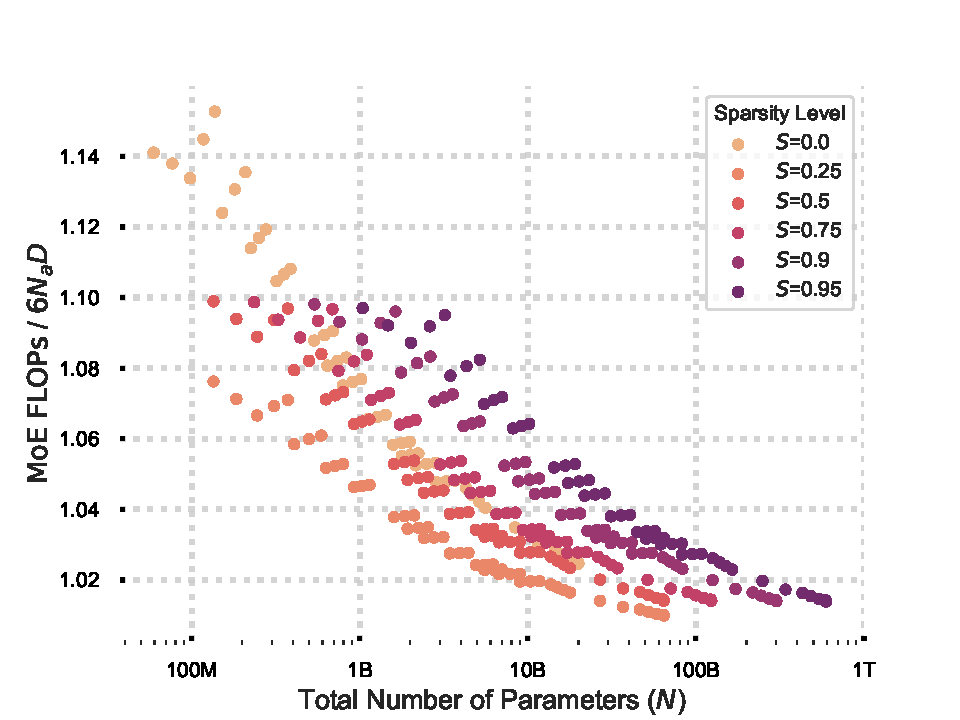
\includegraphics[width=0.8\textwidth]{plots/appendix/app_flop_6nd-v2.pdf}
    \caption{\textbf{Accuracy of $6N_aD$ FLOPs Estimator for MoEs}.
    Ratio of the MoE FLOPs estimator (\Cref{eq:flops}) to the $6N_aD$ estimator as a function of the total number of parameters, for a fixed context length of $D = 2048$, used in our experiments.}
    \label{fig:flop_6nd_v2}
\end{figure}

\begin{comment}
\subsection{Counting Theoretical Flops}
\label{app:count_flops}
Let:
\begin{itemize}
    \item $d_{\text{model}}$ denote the embedding dimension
    \item $G$ denote the granularity (default is 1)
    \item $E_{\text{total}}$ denote the total number of experts
    \item $E_{\text{top-k}}$ denote the number of active experts
    \item $n_{\text{layers}}$ denote the number of layers
    \item $n_{\text{ctx}}$ denote the context length
\end{itemize}

Assume:
\begin{itemize}
    \item All layers are MoE layers
    \item We are using GLU experts instead of MLP experts
    \item The hidden dimension of GLU experts is $d_{\text{ffn}} = 4 \cdot d_{\text{model}}$
\end{itemize}

Forward-and-backward FLOP constants:
\begin{itemize}
    \item For linear projections: $c_L = 6$
    \item For MoE routing: $c_R = 14$ (following ~\citet{ludziejewski2024scaling})
\end{itemize}

FLOPs per token per transformer block:
\begin{itemize}
    \item \textbf{Attention QKV and projection:} $c_L \cdot 2d^2_{\text{model}}$ (with a factor of 2 to account for fewer transformations)
    \item \textbf{Attention logits and values:} $c_L \cdot 2d_{\text{model}} n_{\text{ctx}}$
    \item \textbf{Router:} $c_R \cdot d_{\text{model}} E_{\text{total}}$
    \item \textbf{MoE:} $c_L \cdot 3 d_{\text{ffn}} d_{\text{model}} E_{\text{top-k}} = c_L \cdot \frac{12}{G} d^2_{\text{model}} E_{\text{top-k}}$
    \item \textbf{Final unembedding layer:} $c_L \cdot n_{\text{vocab}} d_{\text{model}}$
\end{itemize}

To simplify, we can skip router FLOPs because $\frac{E_{\text{total}}}{d_{\text{model}}}$ is quite small.
Thus, FLOPs per token simplifies to:
\begin{equation*}
   n_{\text{layers}} \cdot d^2_{\text{model}} \Big( 4c_L + \frac{12c_L}{G} E_{\text{top-k}} + 2c_L \frac{n_{\text{ctx}}}{d_{\text{model}}} + c_L \frac{n_{\text{vocab}}}{d_{\text{model}} n_{\text{layers}}}\Big)
\end{equation*}



% \begin{equation}
%  n_{\text{layers}} \cdot d^2_{\text{model}} \left( 2c_L + \frac{12c_L}{G} E_{\text{top-k}} + 2c_L \frac{n_{\text{ctx}}}{d_{\text{model}}} + c
% \end{equation}




% \Samira{The main problem with this approach is that our cost function is only a function of theoretical flops, whereas in practice costs related to memory and communication can be an important bottleneck, hence the assumption that we infinitely grow total number of parameters and have a fixed training/inference cost for a sparse mixture of expert model as long as number of active parameters is the same is not realistic.}

% \Samira{The fact that the cost function is only a function of theoretical flops is not a big issue for scaling law studies that consider architectures where number of parameters and flops have a linear relation, but in our case this is not the case, as we can increase the total number of parameters almost independently of the number of active parameters which linearly interact with the number of theoretical flops.}

% %Theory
% \paragraph{Theoretical Flops}
% \paragraph{Memory}
% \paragraph{Communication across Experts}

% \begin{equation}
%  \text{Total Cost} = \alpha \times \text{FLOPs} + \beta \times \text{Memory Cost} + \gamma \times \text{Communication Cost}
% \end{equation}
% Adjusting the weights in the equation for total cost involves determining the relative importance of FLOPs, memory cost, and communication cost which depends on hardware and infrastrcure.




% \todo[inline]{In an appendix show what happens if we take memory into account in the cost function (based on some reasonable assumptions that we still need to figure out what they are).}

% Nevertheless, given these results, we  observe that given a limit on the total number of parameters for the model size and the compute budget, there is an optimal sparsity level. In section~\ref{sec:fix_params_vary_sparsity} we further investigate this..
\end{comment}